%----------------------------------------------------------------------------------------
%	PACKAGES AND THEMES
%----------------------------------------------------------------------------------------

\documentclass{beamer}

\mode<presentation> {

\usetheme{default}
\usecolortheme{orchid}

}

\usepackage{graphicx} % Allows including images
\graphicspath{{Fig/}}
\usepackage{booktabs} % Allows the use of \toprule, \midrule and \bottomrule in tables
\usepackage{float}
\usepackage{multirow}
\usepackage{hyperref}
\usepackage{amsmath}

\AtBeginSection[]{
  \begin{frame}
  \vfill
  \centering
  \begin{beamercolorbox}[sep=8pt,center,shadow=true,rounded=true]{title}
    \usebeamerfont{title}\insertsectionhead\par%
  \end{beamercolorbox}
  \vfill
  \end{frame}
}

%----------------------------------------------------------------------------------------
%	TITLE PAGE
%----------------------------------------------------------------------------------------

\title[Calculus]{Mathematics/Statistics Bootcamp} % The short title appears at the bottom of every slide, the full title is only on the title page

\subtitle{Part IV: Basics of Statistical Inference}

\author{Brian Cozzi\inst{1} \and Michael Valancius\inst{1} \and Graham Tierney\inst{1} \and Becky Tang\inst{1}}


\institute[Duke University] % (optional, but mostly needed)
{
  \inst{1}%
  Department of Statistical Science\\
  Duke University
  }
% - Use the \inst command only if there are several affiliations.
% - Keep it simple, no one is interested in your street address.

\date{Graduate Orientation, August 2019}

\begin{document}
\begin{frame}
\titlepage % Print the title page as the first slide
\end{frame}

\begin{frame}
\frametitle{Overview} 
\tableofcontents 
\end{frame}

%----------------------------------------------------------------------------------------
%	PRESENTATION SLIDES
%----------------------------------------------------------------------------------------
\section{Limiting Theorems}
\begin{frame}
\frametitle{The Law of Large Numbers (LLN)}
Suppose $\{X_1,X_2,\ldots\}$ is a sequence of independently and identically distributed (i.i.d.) random variables with $E[X_i] = \mu$. Let $\bar{X}_n = \frac{\sum_{i=1}^n X_i}{n}$ be the sample average. Then:
\begin{itemize}
\item The \textbf{Weak Law}: $\bar{X}_n \xrightarrow[]{p} \mu$ when $n \rightarrow \infty$, that is, for any $\epsilon > 0$,
$$
\lim_{n \rightarrow \infty}P(\vert \bar{X}_n -\mu\vert > \epsilon) = 0.
$$
\item The \textbf{Strong Law}: $\bar{X}_n \xrightarrow[]{a.s.} \mu$ when $n \rightarrow \infty$, that is, 
$$
P\left( \lim_{n \rightarrow \infty}\bar{X}_n =\mu \right) = 1.
$$
\end{itemize}

\end{frame}

\begin{frame}
\frametitle{The Central Limit Theorem (CLT)}
Suppose $\{X_1,X_2,\ldots\}$ is a sequence of independently and identically distributed (i.i.d.) random variables with $E[X_i] = \mu$ and $Var[X_i] = \sigma^2 < \infty$. Let $\bar{X}_n = \frac{\sum_{i=1}^n X_i}{n}$ be the sample average, then as $n \rightarrow \infty$, the random variable $\sqrt{n} (\bar{X}_n - \mu)$ converges in distribution to $N(0,\sigma^2)$:
$$
\sqrt{n} (\bar{X}_n - \mu) \xrightarrow[]{d} N(0,\sigma^2).
$$
\end{frame}

\begin{frame}
\frametitle{Notes on CLT}
\begin{enumerate}

\item The central limit theorem applies regardless of the underlying distribution of the data, so long as the variance of the data is finite and the samples are i.i.d.

\item This is a statement about the sample average, not individual data points.

\item That the distribution of the sample mean is normal is an asymptotic result ($n \rightarrow \infty$).
\end{enumerate}
\end{frame}



\begin{frame}
\frametitle{Simulated Example}
\begin{figure}[H]
\centering
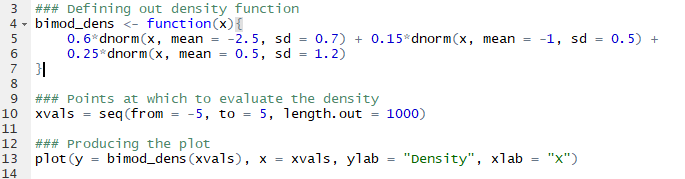
\includegraphics[width=11cm]{bimod_dens_gen.png}
\vspace{0.1 cm}
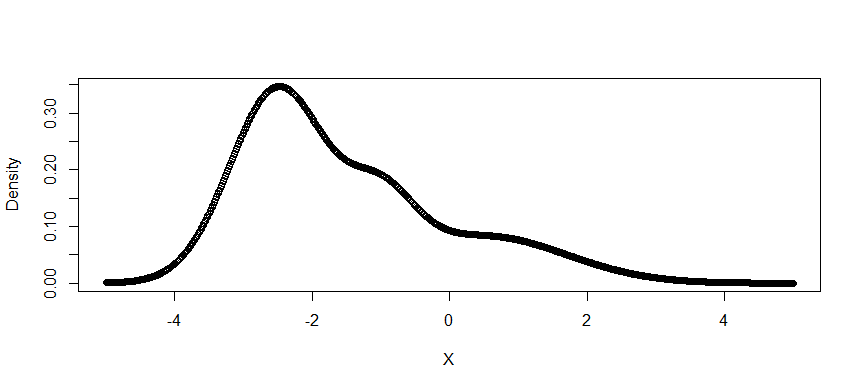
\includegraphics[width=11cm]{bimod_dens_plot.png}
\end{figure}
\end{frame}


\begin{frame}
\frametitle{Simulated Example Cont.}
\begin{figure}[H]
\centering
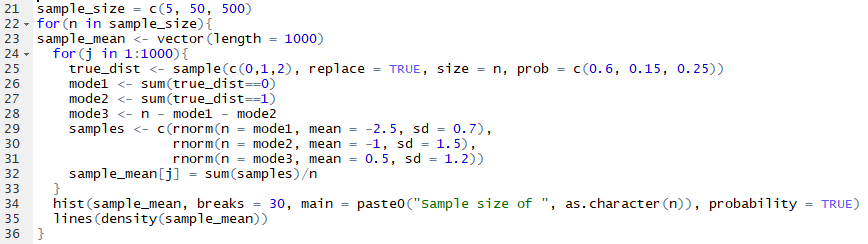
\includegraphics[width=11cm]{bimod_dens_sim.png}
\vspace{0.1 cm}
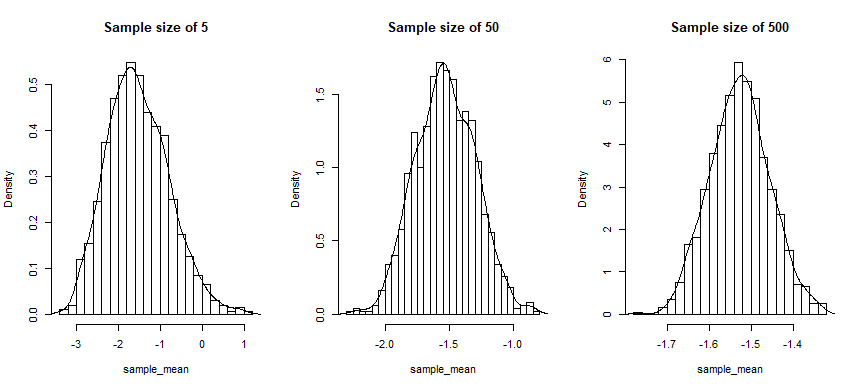
\includegraphics[width=11cm]{bimod_dens_hist.png}
\end{figure}
\end{frame}


\begin{frame}
\frametitle{Mini-exercises}
\begin{enumerate}
\item Rewrite the CLT in terms of the sample sum, $S_n = \sum_{i=1}^n X_i$.
\vspace*{1in}
\item Let $\{X_1,X_2,\ldots,X_n\}$ be a sequence of $n$ independent results from tossing the same fair coin where $X_i = 1$ when the head faces up and $X_i = 0$ otherwise. Let $\bar{X}_n = \frac{\sum_{i=1}^n X_i}{n}$. If $n=100$, estimate the value of 
$$
P(0.4 < \bar{X}_n < 0.6).
$$
% answer: approximately 0.95.
\vspace*{0.7in}
\end{enumerate}
\end{frame}


%------------------------------------------------
\section{Point Estimation}
\begin{frame}
\frametitle{Point Estimation}
\begin{itemize}
\item A \textbf{point estimator} is any function of the sample.
\item \textbf{Estimator} vs. \textbf{Estimate}: The former is a function, while the latter is the realized value of the function (a number) that is obtained when a sample is actually taken.
\end{itemize}
\end{frame}

\begin{frame}
\frametitle{Likelihood Function}
\begin{itemize}
\item If $X_1,\ldots,X_n$ are an i.i.d. sample from a population with pdf or pmf $f(\mathbf{x}|\theta_1,\ldots,\theta_k)$, the \textbf{likelihood function} is
$$
L(\mathbf{\theta}|\mathbf{x}) = L(\theta_1,\ldots,\theta_k|x_1,\ldots,x_n) = \prod_{i=1}^n f(x_i|\theta_1,\ldots,\theta_k).
$$
\item Density function vs Likelihood function. The density function $f(\mathbf{x}|\theta_1,\ldots,\theta_k)$ is a non-negative function that integrates to 1. The likelihood function is a function of the parameter(s) $\theta$ and typically will not integrate to 1.

\item For computational purposes, typically we worked with the log of the likelihood function.

\end{itemize}
\end{frame}

\begin{frame}
\frametitle{Maximum Likelihood Estimators}
\begin{itemize}

\item For each sample point $\mathbf{x}$, let $\hat{\theta}(\mathbf{x})$ be a parameter value at which $L(\mathbf{\theta}|\mathbf{x})$ attains its maximum as a function of $\mathbf{\theta}$, with $\mathbf{x}$ held fixed. A \textbf{maximum likelihood estimator (MLE)} of the parameter $\mathbf{\theta}$ based on a sample $\mathbf{X}$ is $\hat{\theta}(\mathbf{X})$.
\item If the likelihood function is differentiable (in $\theta_i$), \textbf{possible candidates} for the MLE are the values of $(\theta_1,\ldots,\theta_k)$ that satisfy
$$
\frac{\partial}{\partial \theta_i} L(\mathbf{\theta}|\mathbf{x})=0, \quad i=1,\ldots,k.
$$

\item Since $log(\theta)$ is a monotonically increasing function of $\theta$, for any positive valued function $f$, $arg \ max_{\theta} f(x) = arg max_{\theta}$ $log f(x)$. That is, maximizing the log likelihood results in the same MLE estimates as maximizing the likelihood.
\end{itemize}
\end{frame}

\begin{frame}
\frametitle{MLE: Normal Example}
Let $X_1,\ldots,X_n$ be i.i.d. $N(\theta,1)$, and let $L(\theta|\mathbf{x})$ denote the likelihood function. Since maximizing
$$
L(\theta|\mathbf{x}) = \frac{1}{(2\pi)^{n/2}}e^{(-1/2)\sum_{i=1}^n(x_i-\theta)^2},
$$
is equivalent to maximizing $\ln L(\theta|\mathbf{x})$, which reduces to maxizing 
$$
h(\theta)=(-1/2)\sum_{i=1}^n(x_i-\theta)^2,
$$
a quadratic function of $\theta$.
\\~\\
Since $\hat{\theta}=\bar{x}=(\sum_{i=1}^n x_i)/n$ is the global maximum point of $h(\theta)$, it is also the global maximum point of $L(\theta|\mathbf{x})$. Therefore $\hat{\theta}$ is the MLE.
\end{frame}

\begin{frame}
\frametitle{MLE: Exercises}
\begin{enumerate}
\item Let $X_1,\ldots,X_n$ be i.i.d. samples from the uniform distribution $U(0,\theta)$, $\theta > 0$. Find the MLE of $\theta$.
% answer: $\max{X_i}$
\vspace*{1in}
\item Let $X_1,\ldots,X_n$ be i.i.d. $\text{Bernoulli}(p)$. Find the MLE of $p$.
% answer: the sample mean $\sum_{i=1}^n X_i/n$.
\vspace*{1in}
\end{enumerate}
\end{frame}

\begin{frame}
\frametitle{The Invariance Property of MLEs}
\begin{theorem}
If $\hat{\theta}$ is the MLE of $\theta$, then for any function $\tau(\theta)$ of $\theta$, the MLE of $\tau(\theta)$ is $\tau(\hat{\theta})$.
\end{theorem}

\vspace*{0.7in}
A mini-exercise: following ex.2 from above, what is the MLE of $\sqrt{p(1-p)}$?
\end{frame}

\begin{frame}
\frametitle{Further properties of MLEs}
\begin{itemize}
    \item Under certain conditions, the MLE is CAN (\textbf{C}onsistent and \textbf{A}symptotically \textbf{N}ormal). Consistency means that it converges in probability to the true value. The asymptotic normality means that as $n \rightarrow \infty$, $\hat{\theta}_{MLE} \sim Normal \left( \theta, \dfrac{1}{n I(\theta)} \right)$.
    \bigskip
    \item $I(\theta)$ is the Fisher's Information and is defined to be $- \mathrm{E} \left[ \dfrac{\partial^2 log f_{\theta}(X)}{\partial \theta^2} \right]$. If $\theta$ is a scalar, $I(\theta)$ is a scalar, and if $\theta$ is a vector, then $I(\theta)$ is a matrix. 
\end{itemize}
\end{frame}


\begin{frame}
\frametitle{Mean Squared Error (MSE) and Bias}
\begin{itemize}
\item The \textbf{mean squared error (MSE)} of an estimator $W$ of a parameter $\theta$ is defined by $E_{\theta}(W-\theta)^2$.
\item The \textbf{bias} of a point estimator $W$ of a parameter $\theta$ is $\text{Bias}_{\theta}W=E_{\theta}W-\theta$, and an estimator is called \textbf{unbiased} if $E_{\theta}W=\theta$ for all $\theta$.
\item Relationship between MSE and bias:
$$
E_{\theta}(W-\theta)^2 = \text{Var}_{\theta}W + (\text{Bias}_{\theta}W)^2.
$$
\item If $W$ is an unbiased estimator of $\theta$,
$$
E_{\theta}(W-\theta)^2 = \text{Var}_{\theta}W.
$$
\end{itemize}
\end{frame}

\begin{frame}
\frametitle{MSE and Bias: An Exercise}
Let $X_1,\ldots,X_n$ be i.i.d. $N(\mu,\sigma^2)$, $\bar{X}=(\sum_{i=1}^n X_i)/n$ be the sample mean, and $S^2=\sum_{i=1}^n (X_i-\bar{X})^2/(n-1)$ be the sample variance. Verify that $\bar{X}$ and $S^2$ are unbiased estimators for $\mu$ and $\sigma^2$, respectively, and compute their MSEs.\\
(Note: if $Y \sim \chi^2_k$, then $\text{Var}(Y)=2k$.)
%\\ answer: $E(\bar{X}-\mu)^2=\frac{\sigma^2}{n}$, $E(S^2-\sigma^2)^2=\frac{2\sigma^4}{n-1}$.
\vspace*{0.6in}

If we adopt the MLE estimator $\hat{\sigma}^2$ for $\sigma^2$ instead, where $\hat{\sigma}^2=\sum_{i=1}^n (X_i-\bar{X})^2/n$. What is the MSE of $\hat{\sigma}^2$ ?
%\\ answer: $\left(\frac{2n-1}{n^2}\right)\sigma^4$
\vspace*{0.6in}
\end{frame}

% \begin{frame}
% \frametitle{Uniform Minimum Variance Unbiased Estimators}
% \begin{itemize}
% \item If an estimator $W^*$ of $\tau(\theta)$ satisfies $E_{\theta}W^* = \tau(\theta)$ for all $\theta$ and, for any other estimator $W$ with $E_{\theta}W = \tau(\theta)$, we have $\text{Var}_{\theta}W* \leq \text{Var}_{\theta}W$ for all $\theta$, then \textbf{$W^*$} is called a \textbf{uniform minimum variance unbiased estimator (UMVUE) of $\tau(\theta)$}.
% \item Let $T$ be a complete and sufficient statistic for a parameter $\theta$, and let $\phi(T)$ be an estimator based only on $T$ and unbiased for $\tau(\theta)$. Then $\phi(T)$ is the UMVUE of $\tau(\theta)$.
% \end{itemize}
% \end{frame}

\begin{frame}
\frametitle{Review Exercises: Morning Session}
\begin{columns}[t]
\column{.47\textwidth}
1. Let $X_1,X_2,\ldots,X_n$ be i.i.d. $\text{Poisson}(\lambda)$. Let $Y_n = (\sum_{i=1}^n X_i -n\lambda)/\sqrt{n}$. When $n$ is large, $Y_n$ is approximately a normal variable with mean $\mu$ and variance $\sigma^2$. What are $\mu$ and $\sigma^2$ ?

\column{.47\textwidth}
2. Let $X_1,X_2,\ldots,X_n$ be i.i.d. $\text{Exp}(\beta)$ with pdf $f(x)=\beta e^{-\beta x} (x > 0)$. Show that $\bar{X} = \sum_{i=1}^n X_i/n$ is a sufficient statistic for $\beta$, and find the MLE of $\beta$.
\\~\\
3. Let $X$ be a sample from $N(0,\sigma^2)$. Find an unbiased estimator of $\sigma^2$.

\end{columns}
\end{frame}

%------------------------------------------------

\section{Hypothesis Testing}

%\begin{frame}
%\frametitle{Intro to Hypothesis Testing}
%\href{https://youtu.be/VK-rnA3-41c}{\textbf{Video tutorial}, %by \textit{mathtutordvd}}
%\end{frame}

%\begin{frame}
%\frametitle{Challenge Exercises: Morning Session}
%\end{frame}

\begin{frame}
\frametitle{Hypothesis Testing}
\begin{itemize}
    \item In hypothesis testing, a default theory, the null hypothesis, is proposed, and we see if the data provides sufficient evidence to reject this hypothesis.
    \item If we do not reject the null hypothesis, we are said to retain the null hypothesis (sometimes referred to as accepting or failing to reject the null).
    
\end{itemize}
    
\end{frame}

\begin{frame}
\frametitle{Hypothesis Testing: Likelihood Ratio Tests}
Let $\theta = (\theta_1...\theta_q, \theta_{q + 1},...\theta_r)$, while $\Theta_0$ consists of all possible parameter values ($\theta)$ such that $(\theta_{q+1}...\theta_{r}) = (\theta_{0,q+1}...\theta_{0,r})$,

\begin{block}{Remark about terminology}
As a reminder, a parameter is a value that is passed 
in a probability model. For example, in the normal distribution, the parameter, $\theta$, is a vector containing the mean $\mu$ and the variance $\sigma^2$. $\theta$ can take on values in $\Theta$, which is referred to as the parameter space.
\end{block}

\newline
The \textbf{likelihood ratio test statistic} is defined as 
$$
\lambda = 2* log \left( \dfrac{\sup_{\Theta} L(\mathbf{\theta}|\mathbf{x})}{\sup_{\Theta_0)} L(\mathbf{\theta}|\mathbf{x})} \right) = 2* log \left(\dfrac{L(\hat{\theta}) | x}{L(\hat{\theta_0}) | x}.\right)
$$
The \textbf{likelihood ration test} is to reject $H_0$ when $\lambda$ > \chi^2_{r-q, \alpha}.

\end{frame}

%\begin{frame}
%\frametitle{LRT and Sufficiency}
%\begin{theorem}
%If $T(\mathbf{X})$ is a sufficient statistic for $\theta$ and %$\lambda^*(t)$ and $\lambda(\mathbf{x})$ are the LRT statistics based on %$T$ and $\mathbf{X}$, respectively, then %$\lambda^*(T(\mathbf{x}))=\lambda(\mathbf{x})$ for every $\mathbf{x}$ in %the sample space.
%\end{theorem}
%\end{frame}

\begin{frame}
\frametitle{An Exercise: Normal LRT}
Let $X_1,\ldots,X_n$ be i.i.d. $N(\theta,1)$. Consider the test $H_0: \theta=\theta_0$ versus $H_1: \theta \neq \theta_0$. Find the LRT statistic and derive the form of the rejection region.
\\~\\
%Answer: $\lambda(\mathbf{x})=\exp[-n(\bar{x}-\theta_0)^2/2]$, and the rejection region $\{\mathbf{x}: \lambda(\mathbf{x})\leq c\}$ can be written as $\{\mathbf{x}:\vert \bar{x}-\theta_0\vert \geq \sqrt{-2(\log c)/n}\}$.
\end{frame}

\begin{frame}
\frametitle{Test Errors and Power Function}
\begin{itemize}
\item Type I Error and Type II Error:
\begin{table}
\centering
\begin{tabular}{cc|c|c|}
\toprule
 &  & \multicolumn{2}{|c|}{Decision}\\
 &  & Accept $H_0$ & Reject $H_0$ \\
\hline 
\multirow{2}{*}{Truth} & $H_0$ & Correct decision & Type I Error\\
\cline{3-4}
 & $H_1$ & Type II Error & Correct decision\\
\bottomrule
\end{tabular}
\end{table}
\bigskip
\item Suppose $R$ denotes the rejection region for a test, then the probability of a Type I Error is $P(\mathbf{X}\in R|H_0)$, and the probability of a Type II Error is $P(\mathbf{X}\in R^c|H_1)=1-P_{\theta}(\mathbf{X}\in R|H_1)$.
\item A level-$\alpha$ test is one such that $P(\mathbf{X}\in R|H_0) \leq \alpha$.
\end{itemize}
\end{frame}

%\begin{frame}
%\frametitle{An Exercise: Binomial}
%Let $X \sim \text{Binomial}(5,\theta)$. Consider the test $H_0: \theta \leq 1/2$ versus $H_1: \theta > 1/2$. If we adopt the test that rejects $H_0$ only if $X=5$ is observed. What is the power function of this test? How small is the probability of Type I Error? For what values of $\theta$ is the probability of Type II Error less than $\frac{1}{2}$?
\\~\\
%Answer: $\beta(\theta)=\theta^5$. $P(\text{Type I Error})\leq (1/2)^5$. $\theta > (1/2)^{1/5}$, which is approximately 0.87.
%\end{frame}

%\begin{frame}
%\frametitle{p-values}
%\textbf{Definition 1:}\\
%A \textbf{p-value} $p(\mathbf{X})$ is a test statistic satisfying $0 \leq p(\mathbf{x}) \leq 1$ for every sample point $\mathbf{x}$. A p-value is \textbf{valid} if, for every $\theta \in \Theta_0$ and every $0 \leq \alpha \leq 1$,
%$$
%P_{\theta}(p(\mathbf{X}) \leq \alpha) \leq \alpha.
%$$
%\begin{itemize}
%\item If we observe $\mathbf{X} = \mathbf{x}$, then for any $\alpha \geq p(\mathbf{x})$, a level $\alpha$ test rejects $H_0$;
%\item p-value is essentially a summary statistic of the data. Small values of $p(\mathbf{X})$ give evidence that $H_1$ is true.
%\end{itemize}
%\end{frame}

%\begin{frame}
%\frametitle{p-values (Cont'd)}
%\textbf{Definition 2:}\\
%Let $W(\mathbf{X})$ be a test statistic such that large values of $W$ give evidence that $H_1$ is true. For each sample point $\mathbf{x}$, define
%$$
%p(\mathbf{x}) = \sup_{\theta \in \Theta_0} P_{\theta}(W(\mathbf{X}) \geq W(\mathbf{x})).
%$$
%Then $p(\mathbf{X})$ is a valid p-value.
\\~\\
%\begin{itemize}
%\item ``p-value'': the probability of obtaining a sample %``more extreme'' than the ones observed in the data, assuming %$H_0$ is true.
%\end{itemize}
%\end{frame}

\begin{frame}
\frametitle{p-values}
\textbf{Definition:} \\
A \textbf{p-value}, $p(\textbf{X})$, is a statistics such that:
$$
Pr(t(\textbf{Y}^*) \geq t(\textbf{y}) | H_0)
$$
Breaking down the definition:
\begin{itemize}
    \item $t(\textbf{Y}^*)$: A test statistic (such as $\dfrac{\sqrt{n}(\bar{Y} - \mu)}{\sigma^2}$) that is a function of random data ($\textbf{Y}^*$) that you would get under the null hypothesis.
    \item $t(\textbf{y})$: The same test statistic, but of your observed data.
    \item This is a conditional probability. It is conditioned on the null hypothesis being true.
\end{itemize}
\end{frame}

\begin{frame}{p-values cont.}
In much of hypothesis testing, the procedure is to reject $H_0$ if $p(\textbf{X}) \leq \alpha)$. \\
\\~\\
Thus, the p-value can be thought of as the probability of observing data as or more extreme as the observed data under the null hypothesis.
\\~\\
Under the null hypothesis, $p(\textbf{X})$ follows a uniform distribution: $Pr(p(\textbf{X}) \leq c) = c$.
\end{frame}

\begin{frame}
\frametitle{p-values: An Exercise}
A neurologist is testing the effect of a drug on response time by injecting $100$ rats with a unit dose of the drug, subjecting each to neurological stimulus, and recording its response time. The neurologist knows that the response time for a rat not injected with the drug follows a normal distribution with a mean response time of $1.2$ seconds. The mean of the $100$ injected rats' response times is $1.05$ seconds with a sample standard deviation of $0.5$ seconds. 
\\~\\
Do you suggest that the neurologist conclude that the drug has an effect on response time?
\end{frame}

\begin{frame}
\frametitle{Solution to the Exercise}
Suppose the mean response time for rats injected with the drug is $\mu$, then we want to test
$$
H_0: \mu = 1.2s \text{ (the drug has no effect) }
$$
against
$$
H_1: \mu \neq 1.2s \text{ (the drug has effect) }.
$$
Construct the test statistic (here $\bar{X}$ is the sample mean, and $S$ is the sample standard deviation)
$$
Z = \frac{\bar{X} - 1.2}{S/\sqrt{100}}.
$$
$Z \sim t_{99}$, which is approximately $N(0,1)$. Plug in the observed data, $\bar{x} = 1.05, s = 0.5$, and $z=-3$, so the p-value is approximately $P(\vert W \vert \geq \vert z \vert) = P(\vert W \vert \geq 3) \approx 0.003$ (let $W \sim N(0,1)$).%, suggesting strong evidence that $H_1$ is true.
\end{frame}


%------------------------------------------------
\section{Interval Estimation}
%\begin{frame}
%\frametitle{Interval Estimation}
%\begin{itemize}
%\item An \textbf{interval estimate} of a parameter $\theta$ is any pair of functions, $L(x_1,\ldots,x_n)$ and $U(x_1,\ldots,x_n)$, of a sample that satisfy $L(\mathbf{x}) \leq U(\mathbf{x})$ for all $\mathbf{x} \in \mathcal{X}$. The inference $L(\mathbf{x}) \leq \theta \leq U(\mathbf{x})$ is made once $\mathbf{X} = \mathbf{x}$ is observed. The \textbf{random interval} $[L(\mathbf{X}),U(\mathbf{X})]$ is called an \textbf{interval estimator}.
%\item The \textbf{coverage probability} of an interval estimator $[L(\mathbf{X}),U(\mathbf{X})]$ of a parameter $\theta$ is the probability that the random interval $[L(\mathbf{X}),U(\mathbf{X})]$ covers the true parameter, $\theta$. It is denoted by $P(\theta \in [L(\mathbf{X}),U(\mathbf{X})])$, or $P(\theta \in [L(\mathbf{X}),U(\mathbf{X})]|\theta)$.
%\item The \textbf{confidence coefficient} of an interval estimator $[L(\mathbf{X}),U(\mathbf{X})]$ of a parameter $\theta$ is the infimum of the coverage probabilities for all values of $\theta$, $\inf_{\theta}P(\theta \in [L(\mathbf{X}),U(\mathbf{X})])$.
%\end{itemize}
%\end{frame}

\begin{frame}{Interval Estimation}
\begin{itemize}
\item An \textbf{interval estimate} of a parameter $\theta$ is any pair of functions, $L(x_1,\ldots,x_n)$ and $U(x_1,\ldots,x_n)$, of a sample that satisfy $L(\mathbf{x}) \leq U(\mathbf{x})$ for all $\mathbf{x} \in \mathcal{X}$. The inference $L(\mathbf{x}) \leq \theta \leq U(\mathbf{x})$ is made once $\mathbf{X} = \mathbf{x}$ is observed. The \textbf{random interval} $[L(\mathbf{X}),U(\mathbf{X})]$ is called an \textbf{interval estimator}.
\item We call $C_n = (L(X_1...X_n), \ U(X_1...X_n))$ a $1 - \alpha$ confidence interval if $P_\theta(X \in C_n) \geq 1 - \alpha$ for all $\theta \in \Theta$
\item This is not a probability statement about $\theta$: the interval is the random quantity, not the parameter. Such interpretation will be explored further in a Bayesian context. 
\end{itemize}
\end{frame}

%\begin{frame}
%\frametitle{Interval Estimation: Key Points}
%\begin{enumerate}
%\item The \textbf{interval} is the random quantity, not the parameter; 
%\item \textbf{``Confidence intervals/sets''}: interval estimators with a measure of confidence (a confidence coefficient); eg. a confidence interval/set with confidence coefficient equal to $C$, is called a ``$C$ confidence interval/set''.
%\item The \textbf{coverage probability} is a function of $\theta$, whose true value is unknown, so we can only guarantee the infimum of the coverage probability, the confidence coefficient.
%\end{enumerate}
%\end{frame}

\begin{frame}
\frametitle{A mini-exercise}
Suppose that $X$ is a random sample from a distribution with parameter $\theta$, and $[L(X),U(X)]$ is a 95\% confidence interval of $\theta$. If we observe $X=x$, which of the following statements is correct?
\begin{itemize}
\item[A] The probability that $\theta \in [L(x),U(x)]$ is 0.95;
\item[B] The probability that $\theta \in [L(x),U(x)]$ is either 1 or 0.
\end{itemize}
\end{frame}

% \begin{frame}
% \frametitle{Find Interval Estimators Through Pivot Quantities}
% \begin{itemize}
% \item A random variable $Q(\mathbf{X},\mathbf{\theta})$ is a \textbf{pivot quantity} if the distribution of $Q(\mathbf{X},\mathbf{\theta})$ is independent of all parameters.
% \item Usually, $Q(\mathbf{X},\mathbf{\theta})$ contains both parameters and statistics, but for any set $\mathcal{A}$, $P_{\theta}(Q(\mathbf{X},\mathbf{\theta})\in \mathcal{A})$ does not depend on $\theta$.
% \item The goal is to find a pivot quantity $Q(\mathbf{x},\mathbf{\theta})$ and a set $\mathcal{A}$ such that the set $\{\mathbf{\theta}:Q(\mathbf{x},\mathbf{\theta})\in \mathcal{A}\}$ is a set estimate of $\mathbf{\theta}$.
% \end{itemize}
% \end{frame}

\begin{frame}
\frametitle{Example: Normal Confidence Interval}
If $X_1,\ldots,X_n$ are i.i.d. $N(\mu,\sigma^2)$ with $\sigma^2$ known, then $Z=(\bar{X}-\mu)/(\sigma/\sqrt{n})$ is a standard normal variable ($Z \sim N(0,1)$). Then a confidence interval of $\mu$ can be
$$
\{\mu: \bar{x}-a\frac{\sigma}{\sqrt{n}} \leq \mu \leq \bar{x}+a\frac{\sigma}{\sqrt{n}}\},
$$
where $a$ is a constant. \\
If $\sigma^2$ is unknown, then $T_{n-1}=(\bar{X}-\mu)/(S/\sqrt{n}) \sim t_{n-1}$ which is independent of $\mu$. Thus, for any given $\alpha \in (0,1)$, a $1-\alpha$ confidence interval of $\mu$ is given by
$$
\{\mu: \bar{x}-t_{n-1,(1-\alpha/2)}\frac{s}{\sqrt{n}} \leq \mu \leq \bar{x}+t_{n-1,(1-\alpha/2)}\frac{s}{\sqrt{n}}\},
$$
where $t_{df,p}$ is the $p\times 100\%$th quantile of a student-$t$ distribution with $df$ degrees of freedom.
\end{frame}


\end{document}